
\documentclass{article}
\usepackage[utf8]{inputenc} 
\usepackage[T1]{fontenc}
\usepackage{lmodern}
\usepackage[french]{babel}
\usepackage{graphicx}
\usepackage{amsmath}
\usepackage{amssymb}
\usepackage{booktabs}
\usepackage{array}
\usepackage{hyperref}
\usepackage{float}
\usepackage{geometry}
\usepackage[none]{hyphenat} % Désactive complètement la césure
\usepackage{algorithm}      % Pour l'environnement algorithm
\usepackage{algpseudocode}  % Pour les structures algorithmiques
\usepackage[french]{babel}
\usepackage{array}
\usepackage{xcolor}
\usepackage{hyperref}
\usepackage{booktabs}
\usepackage{tabularx}

\DeclareMathOperator*{\argmax}{argmax}
\geometry{margin=2.5cm}
\usepackage{titlesec}
\titleformat{\section}{\Large\bfseries}{\thesection}{1em}{}
\geometry{a4paper, margin=1in} 

\begin{document} 
\title{Optimisation des Flux dans un Entrepôt Intégrant un Algorithme d'Apprentissage par Renforcement}

\author{
    Dr. Bienvenue N.M. MOUALE\thanks\ \ ,
    Université Nangui Abrogoua,
    \texttt{bmouale@mail.ru}
    \and
    Jean Martin,
    Université Nangui Abrogoua ,
    \texttt{jean.martin@polytechnique.edu}
   \and
    Jean Martin,
    Université Nangui Abrogoua ,
    \texttt{jean.martin@polytechnique.edu}
}
 
\date{Juillet, 2025}
\maketitle
%\begin{abstract}
\section*{Résumé}
Dans le secteur du e-commerce, la gestion des entrepôts est un maillon critique de la chaîne logistique. Ce document présente une solution d’optimisation dynamique des flux intralogistiques par l’intelligence artificielle, en particulier à travers un algorithme d’apprentissage par renforcement (Reinforcement Learning - RL).

\section*{Introduction}
Dans le secteur du e-commerce, la gestion des entrepôts est un maillon critique de la chaîne logistique, notamment face à la volatilité de la demande, à la pression sur les délais de livraison et à la multiplication des références produits. Ces contraintes s'accompagnent de difficultés croissantes en matière de mobilité interne, de complexité opérationnelle, et imposent une rigueur de gestion accrue, avec pour objectif constant la recherche de gains de productivité, de temps et de coûts.

Dans ce contexte, l'optimisation dynamique des flux intralogistiques devient une priorité stratégique. L'utilisation de l'intelligence artificielle, et plus particulièrement des algorithmes d'apprentissage par renforcement (Reinforcement Learning RL), permet de développer des systèmes adaptatifs capables d'apprendre en continu à partir des interactions avec leur environnement pour prendre des décisions optimales en temps réel.

L'objectif principal de ce travail est de concevoir une solution d'optimisation des flux dans un entrepôt e-commerce en intégrant un algorithme d'apprentissage par renforcement. Cette approche vise à améliorer l'efficacité des déplacements, à réduire les temps de préparation des commandes et à minimiser les coûts d'exploitation.

Les objectifs spécifiques sont les suivants :
\begin{itemize}
    \item Énoncer le problème à résoudre
    \item Modéliser l'environnement de l'entrepôt sous forme d'un problème de décision séquentielle adapté à l'apprentissage par renforcement
    \item Définir les états, actions et fonctions de récompense représentatifs des objectifs logistiques
    \item Implémenter un algorithme RL adapté (Q-Learning, DQN, etc.) à la dynamique de l'entrepôt
    \item Évaluer les performances de la solution par simulation et comparaison aux modèles réalisations avec des algorithmes traditionnels tel que l'algorithme de Dijkstra
\end{itemize}
%\end{abstract}

\section{État de l'art}
L'optimisation des flux dans les entrepôts représente un enjeu stratégique pour améliorer l'efficacité logistique. Les recherches dans ce domaine ont porté sur la préparation de commandes, le stockage dynamique ou encore la gestion du trafic robotisé, en mobilisant des approches traditionnelles (programmation linéaire, heuristiques) mais aussi des techniques d'intelligence artificielle, notamment l'apprentissage par renforcement (RL).

Des travaux comme ceux de \textbf{Cals et al. [3]} ont appliqué le \textbf{Q-Learning} et les \textbf{Deep Q-Networks (DQN)} pour optimiser les itinéraires de picking dans des entrepôts automatisés. \textbf{Dunn et al. [4]} ont exploré les systèmes de picking basés sur le RL dans des environnements de type Robotic Mobile Fulfillment System. Par ailleurs, \textbf{Krnjaic et al. [6]} ont étudié le \textbf{multi-agent reinforcement learning (MARL)} pour coordonner plusieurs robots en environnement partagé, et \textbf{Zhou et al. [7]} ont introduit un modèle de récompense segmentée pour optimiser la navigation robotique en entrepôt. Des simulations réalistes via \textbf{OpenAI Gym}, \textbf{FlexSim} ou \textbf{RWARE} (AltenBern, 2023) sont également utilisées pour entraîner les agents dans des contextes proches du réel.

Cependant, ces recherches souffrent de plusieurs limitations : difficulté de généralisation à des entrepôts dynamiques [9] modélisations statiques, coût computationnel élevé des modèles de RL profonds, ou encore manque de validation sur des systèmes physiques. De plus, les fonctions de récompense utilisées restent souvent trop simplistes, sans intégrer des paramètres opérationnels complexes tels que la priorité des commandes ou la congestion [5].

Le présent travail se démarque par une approche intégrée combinant \textbf{modélisation sur mesure}, \textbf{fonction de récompense multicritère}, et \textbf{évaluation dans un environnement simulé réaliste}. L'objectif est d'optimiser simultanément le temps de traitement, les déplacements et les conflits de ressources. Cette démarche vise une \textbf{meilleure applicabilité industrielle}, avec une ouverture vers l'intégration dans des systèmes WMS (Warehouse Management System) ou des jumeaux numériques.

\section{Optimisation des flux dans un entrepôt e-commerce}
\subsection{Problème à résoudre}
Le problème à résoudre est d'optimiser les flux dans un entrepôt ayant la forme suivante :

\begin{figure}[h]
    \centering
    \includegraphics[width=0.8\textwidth]{image1.png} 
    \caption{Schéma de l'entrepôt}
    \label{fig:Schéma de l'entrepôt}
\end{figure}


On supposera que l'entrepôt appartient à une entreprise e-commerce à l'image de Amazon, Alibaba, Aliexpres, Djumia ou encore Ozon russe qui vend des produits à une clientèle variée. Les produits sont stockés à l'intérieur dans 12 emplacements différents, identifiés par les lettres suivantes de A à L :

\begin{figure}[h]
    \centering
    \includegraphics[width=0.8\textwidth]{image2.png} 
    \caption{Emplacements de stockage}
    \label{fig:Emplacements de stockage}
\end{figure}
Alors que les commandes sont effectuées par les clients en ligne, un robot autonome se déplace dans l'entrepôt afin de collecter les produits pour les livraisons ultérieures. Voici à quoi cela ressemble :
\begin{figure}[h]
    \centering
    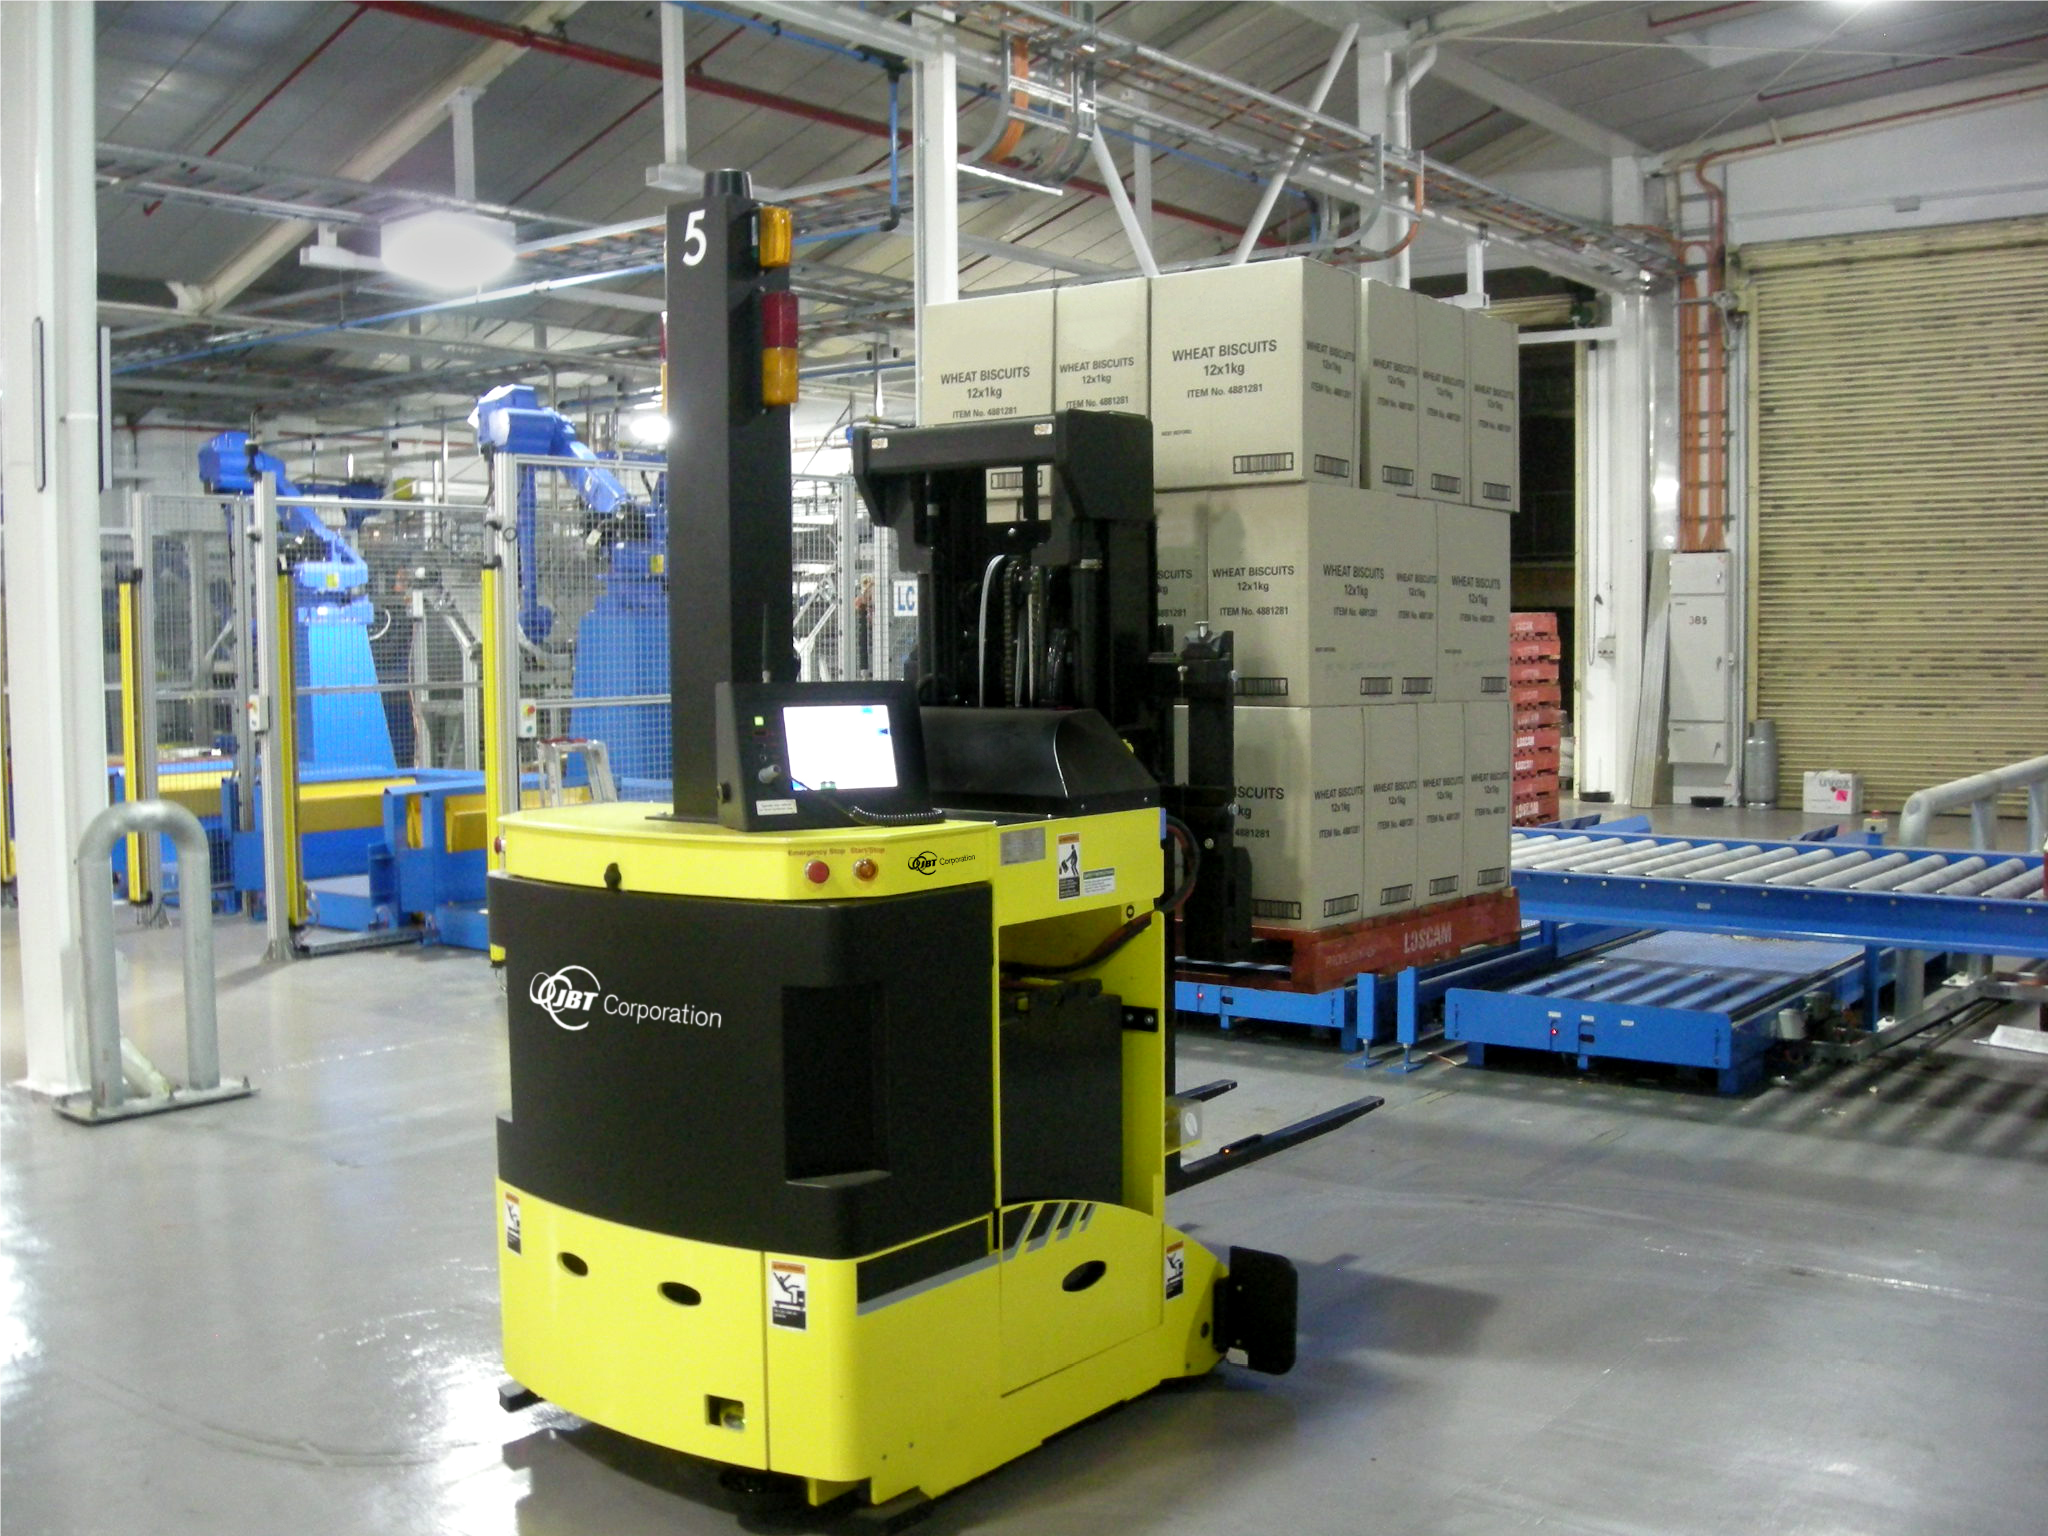
\includegraphics[width=0.8\textwidth]{image3.png} 
    \caption{Robot d'entrepôt autonome}
    \label{fig:Robot d'entrepôt autonome}
\end{figure}

Les 12 emplacements que nous avons définis sont au préalable tous reliés à un système informatique qui indexe en temps réel les priorités de collecte des produits pour ces 12 emplacements. Par exemple, à un temps donné t, il donnera le classement suivant :

\begin{table}[H]
    \centering
    \begin{tabular}{|c|c|}
        \hline
        Niveau de priorité & Emplacement \\
        \hline
        1 & G \\
        2 & K \\
        3 & L \\
        4 & J \\
        5 & A \\
        6 & I \\
        7 & H \\
        8 & C \\
        9 & B \\
        10 & D \\
        11 & F \\
        12 & E \\
        \hline
    \end{tabular}
    \caption{Priorité des emplacements}
\end{table}

L'emplacement G a la priorité 1 (priorité absolue), car il contiendrait un produit qui doit être collecté et livré immédiatement. Notre robot d'entrepôt autonome doit se déplacer vers l'emplacement G \textbf{par l'itinéraire le plus court selon l'endroit où il se trouve}. \textbf{Notre objectif est de développer une IA nommé Prio  indiquant l'itinéraire le plus court entre la position du robot et l’emplacement de collecte}. Toutefois, les emplacements K et L figurent parmi les trois premières priorités. Par conséquent, nous voulons intégrer une option pour passer par des emplacements intermédiaires avant d'atteindre l'emplacement final.

\subsection{Définition de la méthodologie et de l'environnement d'étude}
Afin de résoudre le problème énoncé plus haut, nous allons créer une IA qui utilise des algorithmes de Q-Learning, de Deep Q-Learning et d'autres algorithmes du Machine Learning. Lors de la création de cette IA, la première chose que nous ferons sera de définir l'environnement.

Cela nécessite les trois éléments suivants :
\begin{itemize}
    \item Définir les états
    \item Définir les actions
    \item Définir les récompenses
\end{itemize}

\subsubsection{Définition des états}
L'état d'entrée est simplement l'emplacement où se trouve notre Robot d'Entrepôt autonome à un temps défini t. Cependant, puisque nous implémenterons notre IA avec des équations, nous encoderons les noms d'emplacement (A, B, C,...) avec des numéros d'index selon le schéma suivant :

\begin{table}[H]
    \centering
    \begin{tabular}{|c|c|}
        \hline
        Emplacement & État \\
        \hline
        A & 0 \\
        B & 1 \\
        C & 2 \\
        D & 3 \\
        E & 4 \\
        F & 5 \\
        G & 6 \\
        H & 7 \\
        I & 8 \\
        J & 9 \\
        K & 10 \\
        L & 11 \\
        \hline
    \end{tabular}
    \caption{Encodage des emplacements}
\end{table}
Il y a une raison spécifique pour laquelle nous encodons les états avec des index de 0 à 11 au lieu d'autres nombres entiers. La raison est que nous travaillons avec des matrices. Une matrice de récompenses et une matrice de Q-Values. Chaque ligne/colonne de ces matrices correspond à un emplacement spécifique. Par exemple la 1re ligne de chaque matrice qui a l'index 0 correspond à l'emplacement A ; la 2e ligne/colonne qui a l'index 1 correspond à l'emplacement B, etc. 

\subsubsection{Définition des actions}
Les actions sont simplement les mouvements potentiels du robot pour aller d'un emplacement à l'autre. Par exemple, disons que le robot est à l'emplacement J, les actions possibles à exécuter sont I, F ou K. Nous allons encoder ces actions avec les mêmes index que pour les états. Ainsi, la liste totale des actions que l'IA peut exécuter globalement est la suivante :
\[ \text{Actions} = \{0,1,2,3,4,5,6,7,8,9,10,11\} \]

Évidemment, quand le robot est dans un emplacement précis, il y a certaines actions que l'IA ne peut pas exécuter. Suivant l'exemple précédent, si le robot se trouve à l'emplacement J, il peut exécuter les actions 5, 8 et 10, mais pas les autres. Nous veillerons à attribuer une récompense de 0 aux actions qu'il ne peut pas exécuter et une récompense de 1 aux actions qu'il peut exécuter. Cela nous amène aux récompenses.

\subsubsection{Définition des récompenses}
La dernière chose qui reste pour créer notre environnement est de définir un système de récompenses.  Plus précisément, une fonction de récompense R qui prend comme entrées un état s et une action a, et génère une récompense numérique que l'IA obtiendra en exécutant l'action a dans l'état s :

\[ R: (\text{état}, \text{action}) \rightarrow r \in \mathbb{R} \]

Notre tâche sera donc de concevoir une fonction mathématique pour notre étude de cas énoncé. Pour ce faire, nous allons procéder de la manière suivante : 
Puisqu'il y a un nombre discret et fini d'états (index 0 à 11) ainsi qu'un nombre discret et fini d'actions (mêmes index 0 à 11), la meilleure façon de concevoir notre fonction de récompense R est de faire une matrice. Notre fonction de récompense sera exactement une matrice de 12 lignes et 12 colonnes dont les lignes correspondent aux états et les colonnes correspondent aux actions. Ainsi, dans notre fonction  \[ R: (\text{s}, \text{a}) \rightarrow r \in \mathbb{R} \] s sera l'index de ligne de la matrice, a sera l'index de colonne de la matrice et r sera la cellule d'index (s; a) dans la matrice. Par conséquent, pour définir notre fonction de récompense, nous devons simplement remplir cette matrice avec les récompenses numériques. Comme indiqué ci-dessus, nous devons d'abord attribuer pour chacun des 12 emplacements une récompense : 0 aux actions que le robot ne peut pas exécuter et 1 aux actions que le robot peut exécuter. En faisant cela pour chacun des 12 emplacements, nous obtiendrons une matrice de récompenses. Nous allons la créer étape par étape en commençant par l'emplacement A. Lorsque le robot se trouve à l'emplacement A, il ne peut se rendre qu'à l'emplacement B. Puisque l'emplacement
A a l'index 0 (1ere ligne de la matrice) et l'emplacement B a l'index 1 (2e colonne de la matrice), la 1ere ligne de la matrice de récompenses aura un 1 dans la 2e colonne et un 0 dans toutes les autres. Passons maintenant à l'emplacement B. Lorsque le robot se trouve à l'emplacement B, il ne peut se rendre qu'à trois emplacements différents : A, C et F. Puisque B a l'index 1 (2e ligne) et A, C, F ont les index respectifs 0, 2, 5 (1re, 3e et 6e colonne), alors la 2e ligne de la matrice de récompenses aura 1 sur les colonnes 1, 3, 6 et 0 sur toutes les autres colonnes. En faisant ainsi pour tous les autres emplacements, nous obtenons notre matrice de récompenses finale.

\begin{table}[H]
    \centering
    \begin{tabular}{|c|c|c|c|c|c|c|c|c|c|c|c|c|}
        \hline
        & A & B & C & D & E & F & G & H & I & J & K & L \\
        \hline
        A & 0 & 1 & 0 & 0 & 0 & 0 & 0 & 0 & 0 & 0 & 0 & 0 \\
        B & 1 & 0 & 1 & 0 & 0 & 1 & 0 & 0 & 0 & 0 & 0 & 0 \\
        C & 0 & 1 & 0 & 0 & 0 & 0 & 1 & 0 & 0 & 0 & 0 & 0 \\
        D & 0 & 0 & 0 & 0 & 0 & 0 & 0 & 1 & 0 & 0 & 0 & 0 \\
        E & 0 & 0 & 0 & 0 & 0 & 0 & 0 & 0 & 1 & 0 & 0 & 0 \\
        F & 0 & 1 & 0 & 0 & 0 & 0 & 0 & 0 & 0 & 1 & 0 & 0 \\
        G & 0 & 0 & 1 & 0 & 0 & 0 & 0 & 1 & 0 & 0 & 0 & 0 \\
        H & 0 & 0 & 0 & 1 & 0 & 0 & 1 & 0 & 0 & 0 & 0 & 1 \\
        I & 0 & 0 & 0 & 0 & 1 & 0 & 0 & 0 & 0 & 1 & 0 & 0 \\
        J & 0 & 0 & 0 & 0 & 0 & 1 & 0 & 1 & 0 & 0 & 1 & 0 \\
        K & 0 & 0 & 0 & 0 & 0 & 0 & 0 & 0 & 0 & 1 & 0 & 1 \\
        L & 0 & 0 & 0 & 0 & 0 & 0 & 0 & 1 & 0 & 0 & 1 & 0 \\
        \hline
    \end{tabular}
    \caption{Matrice de récompenses initiale}
\end{table}
Nous venons de définir les récompenses en créant cette matrice de récompenses. Généralement, c'est la façon dont nous définissons le système de récompenses lorsque nous faisons du Q-Learning avec un nombre fini d'entrées et d'actions. Il nous reste à présent l'attribution des récompenses élevées aux emplacements prioritaires par le biais d'un système informatique qui restitue les priorités de collecte des produits pour chacun des 12 emplacements. Par conséquent, puisque l'emplacement G est la priorité absolue, le système informatique mettra à jour la matrice de récompenses en attribuant une récompense élevée dans la cellule (G,G) :

\begin{table}[H]
    \centering
    \begin{tabular}{|c|c|c|c|c|c|c|c|c|c|c|c|c|}
        \hline
        & A & B & C & D & E & F & G & H & I & J & K & L \\
        \hline
        A & 0 & 1 & 0 & 0 & 0 & 0 & 0 & 0 & 0 & 0 & 0 & 0 \\
        B & 1 & 0 & 1 & 0 & 0 & 1 & 0 & 0 & 0 & 0 & 0 & 0 \\
        C & 0 & 10 & 0 & 0 & 0 & 0 & 1 & 0 & 0 & 0 & 0 & 0 \\
        D & 0 & 0 & 0 & 0 & 0 & 0 & 0 & 1 & 0 & 0 & 0 & 0 \\
        E & 0 & 0 & 0 & 0 & 0 & 0 & 0 & 0 & 1 & 0 & 0 & 0 \\
        F & 0 & 1 & 0 & 0 & 0 & 0 & 0 & 0 & 0 & 1 & 0 & 0 \\
        G & 0 & 0 & 1 & 0 & 0 & 0 & \textbf{M} & 1 & 0 & 0 & 0 & 0 \\
        H & 0 & 0 & 0 & 1 & 0 & 0 & 1 & 0 & 0 & 0 & 0 & 1 \\
        I & 0 & 0 & 0 & 0 & 1 & 0 & 0 & 0 & 0 & 1 & 0 & 0 \\
        J & 0 & 0 & 0 & 0 & 0 & 1 & 0 & 1 & 0 & 0 & 1 & 0 \\
        K & 0 & 0 & 0 & 0 & 0 & 0 & 0 & 0 & 0 & 1 & 0 & 1 \\
        L & 0 & 0 & 0 & 0 & 0 & 0 & 0 & 1 & 0 & 0 & 1 & 0 \\
        \hline
    \end{tabular}
    \caption{Matrice de récompenses mise à jour}
\end{table}
C'est ainsi que le système de récompenses fonctionnera avec le Q-Learning. Nous attribuons la récompense la plus élevée (ici M=1000) à l'emplacement de priorité supérieure G. 

\section{Réalisation de la solution d'IA}
La solution d'IA qui résoudra le problème décrit ci-dessus est un modèle Q-Learning. Puisque ce dernier est basé sur les processus décisionnels de Markov (MDPs). Nous commencerons par une définition, puis nous passerons à l'intuition et aux détails mathématiques derrière le modèle Q-Learning.

\subsection{Processus décisionnels de Markov}
Un processus décisionnel de Markov est un tuple $(S, A, T, R)$ où :
\begin{itemize}
    \item $S$ est l'ensemble des différents états. Par conséquent, dans notre étude de cas 
    $$S=\{0,1,2,3,4,5,6,7,8,9,10,11\}$$
    
    \item $A$ est l'ensemble des actions qui peuvent être exécutées à chaque temps $t$. Dans notre étude de cas :
    $$A=\{0,1,2,3,4,5,6,7,8,9,10,11\}$$
    
    \item $T$ s'appelle la règle de transition :
    $$T: (S_t \in S, S_{t+1} \in S, a_t \in A) \longmapsto \mathbb{P}(s_{t+1} | s_t, a_t)$$
    Où $\mathbb{P}(s_{t+1} | s_t, a_t)$ est la probabilité d'atteindre l'état futur $S_{t+1}$ en exécutant l'action $a_t$ dans l'état $s_t$. Donc $T$ est la distribution de probabilité des états futurs au temps $t+1$ étant donné l'état actuel et l'action exécutée au temps $t$. Par conséquent, nous pouvons prévoir l'état futur $s_{t+1}$ en faisant un tirage aléatoire dans cette distribution $T$:
    $$s_{t+1} \sim T(s_t, a_t)$$
    
    Dans notre recherche, la distribution $T$ de notre IA sera une distribution uniforme, ce qui est un choix classique de distribution qui fonctionne très bien en faisant du Q-Learning.
    
    \item $R$ est la fonction de récompense :
    $$R: (s_t \in S, a_t \in A) \longmapsto r_t \in \mathbb{R}$$
    où $r_t$ est la récompense obtenue après avoir exécuté l'action $a_t$ dans l'état $s_t$. Dans notre étude de cas, cette fonction de récompense est exactement la matrice que nous avons créée précédemment.
\end{itemize}

Après avoir défini les processus décisionnels de Markov, il est maintenant important de rappeler qu'il repose sur l'hypothèse suivante : la probabilité de l'état futur $s_{t+1}$ dépend uniquement de l'état actuel $s_t$ et de l'action $a_t$, et ne dépend d'aucun des états et actions précédents. C'est à dire :
$$\mathbb{P}(s_{t+1} | s_0, a_0, s_1, a_1, \dots, s_t, a_t) = \mathbb{P}(s_{t+1} | s_t, a_t)$$

En d'autres termes, un processus décisionnel de Markov n'a pas de mémoire.

En résumé en ce qui concerne les processus décisionnels de Markov. À chaque temps $t$ :
\begin{itemize}
    \item L'IA observe l'état actuel $s_t$.
    \item L'IA exécute l'action $a_t$.
    \item L'IA reçoit la récompense $r_t = R(s_t, a_t)$.
    \item L'IA passe à l'état suivant $s_{t+1}$.
\end{itemize}

Notre tâche revient donc à déterminer à quel moment l'IA sait-elle quelle action exécuter à chaque temps $t$. Pour ce faire, nous devons introduire la fonction de stratégie. La fonction de stratégie $\pi$ est exactement la fonction qui, étant donné l'état $s_t$ indique l'action $a_t$ :
$$\pi: s_t \in S \longmapsto a_t \in A$$

Désignons par $\Pi$ l'ensemble de toutes les fonctions de stratégie possibles. Le choix des meilleures actions à exécuter devient alors une question d'optimisation. En effet, il s'agit de trouver la stratégie optimale $\pi^*$ qui maximise la récompense accumulée :
$$\pi^* = \underset{\pi \in \Pi}{\mathrm{argmax}} \sum_{t \geq 0} R(s_t, \pi(s_t)).$$

Par conséquent, nous devons maintenant trouver cette stratégie optimale $\pi^*$. Pour la résolution de cette équation, nous allons utiliser le Q-Learning.

\subsection{Utilisation du Q-Learning}
\subsubsection{La Q-Value}
À chaque couple d'état et action $(s, a)$, nous allons associer une valeur numérique $Q(s, a)$ :

$$Q: (s_t \in S, a_t \in A) \longmapsto Q(s, a) \in \mathbb{R}$$

Nous dirons que $Q(s, a)$ est \og la Q-value de l'action $a$ exécutée dans l'état $s$\fg.

Pour comprendre l'objectif de cette \og Q-Value \fg, nous devons introduire la \emph{différence temporelle}.

\subsubsection{La Différence temporelle}
Au début $t = 0$, toutes les Q-values sont initialisées à $0$ :
\[
\forall s \in S, a \in A, Q(s, a) = 0
\]

Supposons maintenant que nous soyons au temps $t$, dans un certain état $s_t$. Nous exécutons une action aléatoire $a_t$, ce qui nous amène à l'état $s_{t+1}$ et nous obtenons la récompense $R(s_t, a_t)$.
Nous pouvons maintenant introduire la \emph{différence temporelle} qui est au cœur du Q-Learning. La différence temporelle au temps $t$, désignée par $\text{TD}_t(s_t, a_t)$, est la différence entre :
\begin{itemize}
    \item $R(s_t, a_t) + \gamma \max_a Q(s_{t+1}, a)$, soit la récompense $R(s_t, a_t)$ obtenue en exécutant l'action $a_t$ dans l'état $s_t$, plus la Q-value de la meilleure action exécutée dans l'état futur $s_{t+1}$, actualisée par un facteur $\gamma \in [0, 1]$, appelé \emph{facteur de réduction}.
    
    \item $Q(s_t, a_t)$, soit la Q-value de l'action $a_t$ exécutée dans l'état $s_t$.
\end{itemize}
Ce qui mène à :
\[
\text{TD}_t(s_t, a_t) = R(s_t, a_t) + \gamma \max_a Q(s_{t+1}, a) - Q(s_t, a_t)
\]
\subsection{Importance de la Différence Temporelle $TD_t(s_t, a_t)$ }

La différence temporelle $TD_t(s_t, a_t)$ est comme une récompense intrinsèque. L'IA apprendra les Q-values de manière à ce que :
\begin{itemize}
    \item Si $TD_t(s_t, a_t)$ est élevée, l'IA obtient une « bonne surprise ».
    \item Si $TD_t(s_t, a_t)$ est petite, l'IA obtient une « frustration ».
\end{itemize}

Dans cette mesure, l'IA va itérer certaines mises à jour de Q-values (par une équation appelée \emph{équation de Bellman}) vers des différences temporelles plus élevées.

Par conséquent, dans la dernière étape de l'algorithme du Q-Learning, nous utilisons la différence temporelle pour renforcer les couples (état, action) du temps $t-1$ au temps $t$, selon l'équation suivante :

\[
Q_t(s_t, a_t) = Q_{t-1}(s_t, a_t) + \alpha TD_t(s_t, a_t)
\]

où $\alpha \in \mathbb{R}$ est le \emph{taux d'apprentissage} qui détermine la vitesse à laquelle l'apprentissage des Q-values se fait, ou l'importance des mises à jour des Q-values. Sa valeur est généralement un nombre réel choisi entre $0$ et $1$, comme $0.01$, $0.05$, $0.1$ ou $0.5$. Plus sa valeur est faible, plus les mises à jour des Q-values seront petites et plus le Q-Learning sera long. Plus sa valeur est élevée, plus les mises à jour des Q-values seront importantes et plus le Q-Learning sera rapide.

Cette équation ci-dessus est l'\emph{équation de Bellman} qui est le pilier du Q-Learning.

Ainsi, les Q-values mesurent l'accumulation de surprise ou de frustration associées au couple action et état $(s_t, a_t)$. Dans le cas de surprise, l'IA est renforcée et dans le cas de la frustration, l'IA est affaiblie. C'est pourquoi nous voulons apprendre les Q-values qui donneront à l'IA le maximum de « bonne surprise ».

Par conséquent, la décision de l'action à exécuter dépend principalement de la Q-value $Q(s_t, a_t)$. 
\begin{itemize}
    \item Si l'action $a_t$ exécutée dans l'état $s_t$ est associée à une Q-value élevée $Q(s_t, a_t)$, l'IA aura plus tendance à choisir $a_t$.
    \item Par contre si l'action $a_t$ exécutée dans l'état $s_t$ est associée à une petite Q-value $Q(s_t, a_t)$, l'IA aura moins tendance à choisir $a_t$.
\end{itemize}

Il faut noter qu'il y a plusieurs façons de choisir la meilleure action à exécuter. Lorsque nous sommes dans un état $s_t$, nous pourrions simplement prendre l'action $a_t$ qui maximise la Q-value $Q(s_t, a_t)$:

\[
a_t = \arg\max_a Q(s_{t+1}, a)
\]

Cette solution est la solution \emph{Argmax} et c'est celle que nous avons utilisée dans la résolution du problème posé dans notre recherche.

\subsection{L'algorithme Q-Learning complet}

Il est temps à présent d'étudier l'algorithme d'Intelligence Artificielle permettant de résoudre notre cas d'usage. Résumons les différentes étapes de l'ensemble du processus de Q-Learning :

\begin{itemize}
    \item \textbf{Initialisation} :
    \begin{itemize}
        \item Pour tous les couples d'états $s$ et d'actions $a$, les Q-values sont initialisées à $0$ :
        \[
        \forall s \in S, a \in A, Q_0(s, a) = 0
        \]
        \item Nous commençons dans l'état initial $s_0$. Nous exécutons une action aléatoire pour atteindre le 1er état $s_1$.
    \end{itemize}
    
    \item \textbf{Itérations} ($\mathbf{t \geq 1}$) :
    \begin{itemize}
        \item Nous sélectionnons un état aléatoire $s_t$ parmi nos 12 états possibles :
        \[
        s_t = \text{random}\{0, 1, 2, 3, 4, 5, 6, 7, 8, 9, 10, 11\}
        \]
        
        \item Nous exécutons une action aléatoire $a_t$ qui peut mener à un futur état possible, c.-à-d. $R(s_t, a_t) > 0$ :
        \[
        a_t = \text{random}\{0, 1, \dots, 11\} \quad \text{t.q.} \quad R(s_t, a_t) > 0
        \]
        
        \item Nous atteignons l'état suivant $s_{t+1}$ et nous obtenons la récompense $R(s_t, a_t)$
        
        \item Nous évaluons la différence temporelle $TD_t(s_t, a_t)$ :
        \[
        TD_t(s_t, a_t) = R(s_t, a_t) + \gamma \max_a Q(s_{t+1}, a) - Q(s_t, a_t)
        \]
        
        \item Nous mettons à jour la Q-value en appliquant l'équation de Bellman :
        \[
        Q_t(s_t, a_t) = Q_{t-1}(s_t, a_t) + \alpha TD_t(s_t, a_t)
        \]
    \end{itemize}
\end{itemize}

\textbf{Remarque :} Ce processus est répété un grand nombre de fois (1000 fois dans notre code).

\section{Implémentation de la solution d'Intelligence Artificielle proposée}

Dans cette partie, nous allons expliquer l'implémentation complète du modèle Q-Learning réalisé sur la bas de notre algorithme Prio qui est  la solution de notre problème d'optimisation des flux de stockage dans un entrepôt e-commerce.
Nous définissons les paramètres de notre modèle. Il s'agit de: 
\begin{itemize}
    \item Facteur de réduction ($\gamma$)
    \item Taux d'apprentissage ($\alpha$)
\end{itemize}
Ces paramètres $\alpha$ et $\gamma$ sont les seuls paramètres de l'algorithme du Q-Learning.

 Ensuite nous définissons les récompenses en créant une matrice $R$ dont les lignes correspondent aux états actuels $s_t$, les colonnes aux actions $a_t$ menant à l'état suivant $s_{t+1}$,\  et les cellules contiennent les récompenses $R(s_t, a_t)$. Si une cellule ($s_t$; $a_t$) a 1, cela signifie que nous pouvons exécuter l'action $a_t$  depuis l'état actuel $s_t$ pour atteindre l'état suivant $s_{t+1}$. Si une cellule $R(s_t; a_t)$ a 0, cela signifie que nous ne pouvons pas exécuter l'action at depuis l'état actuel $s_t$ pour atteindre l'état suivant $s_{t+1}$. Nous allons mettre manuellement une récompense élevée ($M$) dans la cellule correspondant à l'emplacement $G$, car c'est l'emplacement prioritaire où le robot autonome doit récupérer les produits. Puisque l'emplacement $G$ a encodé l'état avec l'index 6, nous avons mis une récompense de $M$ dans la cellule de la ligne 6 et de la colonne 6. Ensuite, nous développerons notre solution en implémentant un système automatique pour aller à l'emplacement prioritaire sans avoir à mettre à jour manuellement la matrice de récompenses et en la laissant initialisée avec 0 et 1 comme elle devrait l'être. Ensuite développons la solution d'IA avec le Q-Learning. Pour ce faire, nous allons utiliser l'algorithme de Q-Learning exactement tel qu'il a été fourni dans la section 3.4. Nous commençons donc par initialiser toutes les Q-Values en créant notre matrice de Q-Values contenant des zéros (dans laquelle les lignes correspondent aux états actuels $s_t$, les colonnes aux actions $a_t$\ menant aux états suivants $s_{t+1}$\ et les cellules contiennent les Q-Values $Q(s_t; a_t))$. Enfin, nous implémentons le processus de Q-Learning avec une boucle pour plus de  $M$ itérations, répétant  $M$ fois les étapes du processus de Q-Learning fournies à la fin de la section 3.4.

\begin{figure}[h]
    \centering
    \includegraphics[width=0.8\textwidth]{image4.png} 
    \caption{Matrice de Q-Values après apprentissage}
    \label{fig:Matrice de Q-Values après apprentissage}
\end{figure}

Maintenant que nous avons notre matrice, nous pouvons donc passer à la mise en production, dans laquelle nous calculerons le chemin optimal de n'importe quel point de départ à n'importe quel point final de priorité absolue. L'idée est de mettre en place une fonction "route" qui prendra comme entrées le point de départ où se trouve notre robot autonome à un temps donné et le point d'arrivée où il doit aller en priorité absolue, et qui donnera comme sortie le chemin le plus court dans une liste. Cependant, puisque nous voulons entrer les emplacements avec leurs noms (en lettres), par opposition à leurs états (en index), nous aurons besoin d'un dictionnaire qui associe les états (en index) aux emplacements (en lettres). Pour terminer, nous avons implémenter notre fonction finale "route()" qui aura comme entrées les emplacements de départ et d'arrivée, et qui donne l'itinéraire optimal entre ces deux emplacements. Pour expliquer exactement ce que fera cette fonction route, nous allons énumérer les différentes étapes du processus, en allant de l'emplacement E à l'emplacement $G$ :\\
1. Nous commençons à notre emplacement de départ \textbf{E}.\\
2. Nous obtenons l'état de l'emplacement  \textbf{E} (d'après notre mapping\texttt{location\_to\_state}) est $s_0 = 4$\\
3. Sur la ligne d'index $s_0 = 4$ dans notre matrice de Q-Values, nous trouvons la colonne qui a la Q-Value maximale (703).\\
4. Cette colonne a l'index 8, donc nous exécutons l'action de l'index 8 qui mène à l'état suivant $s_{t+1}$ = 8.\\
5. Nous obtenons l'emplacement de l'état 8, qui selon notre mapping \texttt{location\_to\_state} est $I$. AInsi, notre prochain emplacement est I qui est annexé à notre liste contenant le chemin optimal.\\
6. Nous répétons les 5 étapes précédentes à partir de notre nouveau point de départ I jusqu'à ce que nous atteignions notre destination finale, le point $G$.\\


Bien, nous avons une première version du modèle pratique, nous avons proposer une version  l'améliorer de deux façons :\\
•	Tout d'abord, en automatisant l'attribution de récompense à l'emplacement prioritaire afin que nous n'ayons pas à le faire manuellement. \\
•	Deuxièmement, en ajoutant une fonction (qui inclut l'algorithme complet du Q-Learning (y compris l'étape d'initialisation) qui nous donne la possibilité de passer
par un emplacement intermédiaire avant d'aller à l'emplacement prioritaire. Cet emplacement intermédiaire devrait bien sûr figurer parmi les 3 premiers emplacements prioritaires. Dans notre classement des emplacements prioritaires, le deuxième est $K$. \\
Par conséquent, afin d'optimiser encore plus les flux de stockage, notre robot autonome doit passer par l'emplacement K pour récupérer les produits en route vers l'emplacement
prioritaire $G$. Pour ce faire, il est possible de passer par tout emplacement intermédiaire dans le cadre de notre fonction "route()". Et c'est exactement ce que nous avons mis en place comme deuxième amélioration.\\
Ainsi, notre modèle  nous affichera les résultats graphiques  suivants :
\begin{figure}[h]
    \centering
    \includegraphics[width=0.3\textwidth]{image5.png} 
    \caption{Automatisation de l'attribution de récompense à l'emplacement prioritaire}
    \label{fig:Automatisation de l'attribution de récompense à l'emplacement prioritaire}
\end{figure}

\begin{figure}[htbp]
  \centering
  \begin{minipage}[b]{0.45\textwidth}
    \centering
    \includegraphics[width=\textwidth]{image5.png}
    \caption{Automatisation de l'attribution de récompense avec emplacement intermédiaire}
    \label{fig:Automatisation de l'attribution de récompense avec emplacement intermédiaire}
  \end{minipage}
  \hfill
  \begin{minipage}[b]{0.45\textwidth}
    \centering
    \includegraphics[width=\textwidth]{image5.png}
    \caption{Automatisation de l'attribution de récompense avec emplacement intermédiaire}
    \label{fig:Automatisation de l'attribution de récompense avec emplacement intermédiaire}
  \end{minipage}
\end{figure}


\begin{figure}[htbp]
  \centering
  \begin{minipage}[b]{0.45\textwidth}
    \centering
    \includegraphics[width=\textwidth]{image6.png}
    \caption{Image 1}
    \label{fig:image1}
  \end{minipage}
  \hfill
  \begin{minipage}[b]{0.45\textwidth}
    \centering
    \includegraphics[width=\textwidth]{image6.png}
    \caption{Image 2}
    \label{fig:image2}
  \end{minipage}
\end{figure}


\section{Comparaison des performances avec l'algorithme de Dijkstra}
\subsection{Étude de cas 1 : Trajet sans étape intermédiaire}
\begin{itemize}
    \item Départ : D
    \item Arrivée : A
\end{itemize}

\begin{table}[H]
    \centering
    \begin{tabular}{|l|l|l|}
        \hline
        \textbf{Critère} & \textbf{Q-learning} & \textbf{Dijkstra} \\
        \hline
        \textbf{Trajet} & D → H → G → C → B → A & D → H → G → C → B → A \\
       \hline
        \textbf{Temps estimé} & 25 s & 25 s \\
       \hline
        \textbf{Optimalité} & Oui & Oui \\
        \hline
    \end{tabular}  \\ 
    \caption{Comparaison des algorithmes - Cas 1}
\vspace{0.25cm} 
\hspace{1cm} 
\textbf{Observation :} Les deux algorithmes trouvent le même chemin optimal, ce qui montre que le Q-learning a bien appris la politique optimale pour ce graphe.

\end{table}

\subsection{Étude de cas 2 : Trajet avec étape intermédiaire obligatoire imposée}
\begin{itemize}
    \item Départ : A
    \item Étape : E
    \item Arrivée : D
\end{itemize}

\begin{table}[H]
    %\centering
%\resizebox{\textwidth}{!}{%
    \begin{tabularx}{\linewidth}{|X|X|X|}
        \hline
        \textbf{Critère} & \textbf{Q-learning} & \textbf{Dijkstra} \\
        \hline
        \textbf{Trajet} & A → B → F → J → I → E → I →J → K → L → H → D & A → B → F → J → I → E → I → J → K → L → H → D \\
        \hline
        \textbf{Temps estimé} & 55 s & 55 s \\
        \hline
        \textbf{Optimalité} & Oui (même que Dijkstra) & Oui \\
        \hline
    \end{tabularx} \\
  \caption{Comparaison des algorithmes - Cas 2}
\vspace{0.25cm} 
\hspace{1cm} 
\textbf{Observation :} Encore une fois, les deux algorithmes aboutissent au même chemin, ce qui valide la robustesse du Q-learning même avec une contrainte supplémentaire.
  
\end{table}


\subsection{Analyse critique et comparaison approfondie}
\begin{table}[H]
    \centering
    \begin{tabularx}{\linewidth}{|X|X|X|}
        \hline
        \textbf{Point de comparaison} & \textbf{Q-learning} & \textbf{Dijkstra} \\
        \hline
        \textbf{Type} & Apprentissage par renforcement & Recherche déterministe de plus court chemin \\
   	\hline
        \textbf{Connaissance du graphe} & Apprentissage par essais-erreurs, récompenses & Connaissance complète nécessaire dès le départ \\
   	\hline
        \textbf{Convergence} & Peut nécessiter de nombreux épisodes & Résultat immédiat (single run) \\
  	 \hline
        \textbf{Robustesse} & Peut s'adapter à des changements de l'environnement & Moins flexible (besoin de recalculer en cas de changement) \\
  	 \hline
        \textbf{Complexité} & Peut être plus long à initialiser (learning curve) & Plus rapide dans des petits environnements statiques \\
  	 \hline
        \textbf{Résilience} & Plus tolérant aux environnements stochastiques ou dynamiques & Moins performant si le graphe change fréquemment \\
   	\hline
        \textbf{Application idéale} & Robots autonomes, systèmes adaptatifs, environnements non connus à l'avance & Réseaux fixes, chemins optimaux garantis dans un graphe stable \\
        \hline
    \end{tabularx}
    \caption{Comparaison approfondie des approches}
\end{table}



\subsection{Conclusion  analytique}
Les expérimentations montrent que l'algorithme basé sur le Q-learning peut atteindre un niveau de performance comparable à celui de Dijkstra en termes de chemin optimal et de temps estimé. Toutefois, leur philosophie diffère fondamentalement : Dijkstra est idéal pour des systèmes statiques et bien définis, tandis que l'algorithme basé sur le Q-learning est préférable pour des environnements dynamiques et incertains, grâce à sa capacité d'adaptation par apprentissage.

\section*{Bibliographie}
\begin{enumerate}
    \item Arthur Juliani, 2016, \textit{Simple Reinforcement Learning with Tensorflow (10 Parts)}
    \item Richard Sutton et al., 1998, \textit{Reinforcement Learning I: Introduction}
    \item Cals, M. J., van Houtum, G. J., \& van der Heide, D. (2020). \textit{Reinforcement learning for order batching and sequencing in warehouses.} arXiv preprint arXiv:2006.09507.
    \item Dunn, J., Moshref-Javadi, M., \& Roy, D. (2024). \textit{A reinforcement learning-based model for order picking in robotic mobile fulfillment systems.} arXiv preprint arXiv:2402.03525.
    \item Mahmoudinazlou, M., \& Gharehgozli, A. (2024). \textit{Deep reinforcement learning for picker routing problem.} arXiv preprint arXiv:2408.01656.
    \item Krnjaic, T., Bauer, A., \& Kuehn, W. (2022). \textit{Hierarchical Multi-Agent Reinforcement Learning for Warehouse Logistics.} arXiv preprint arXiv:2212.11498.
    \item Zhou, Y., Ren, Y., \& Liu, H. (2021). \textit{Dual segmented reward model for warehouse robot navigation using reinforcement learning.} Applied Sciences, 12(9), 4703.
    \item Kim, S. J., \& Kang, K. H. (2024). \textit{Performance analysis of multi-agent reinforcement learning algorithms in warehouse environments.} Journal of KIISE, 51(3), 289-300.
    \item Islam, M. M., \& Park, J. H. (2023). \textit{Reinforcement Learning-Based Order Picking System in Warehouses Using FlexSim Simulation and Deep RL.} Algorithms, 16(9), 408.
\end{enumerate}

\end{document}
